\documentclass{ctexart}
\usepackage{graphicx}
\usepackage{subfigure}
\usepackage{hyperref}
\usepackage{subfigure}
\usepackage{geometry}
\geometry{left=2.5cm,right=3.5cm,top=2.5cm,bottom=2.5cm}
\CTEXsetup[format+={\flushleft}]{section}

\begin{document}
\CJKfamily{li}
\title{周报}
\author{刘精昌}
\maketitle

\fangsong
\section*{本周工作}
\begin{enumerate}
  \item 阅读《Automatic Generation of Probabilistic Programming from Time Series Data》,基于Compositional Kernel工作,用概率编程语言$Stan$对相关工作进行描述。
  \item 阅读《Gaussian Process Kernels for Pattern Discovery and Extrapolation》ICML13,论文引入一种gp kernel——spectral mixture (SM) kernel,好处是对一些问题精度较高,最主要是能Pattern Discovery。

      在信号分析等很多问题中,会对原始数据进行傅里叶变换,将时域上的数据转换到频域,通过分析频域上的高峰以得到相关信息。既然关注的是频域的高峰,而gauss mixture分布恰是多峰分布,可以先定义频域上的分布(谱密度)是gauss mixture分布。
      再经由傅里叶反变换,得到\[k\left( \tau  \right) = \sum\limits_{q = 1}^Q {{w_q}\prod\limits_{p = 1}^P {\exp \left( { - 2{\pi ^2}\tau _p^2v_q^{\left( p \right)}} \right)\cos \left( {2\pi {\tau _p}\mu _q^{\left( p \right)}} \right)} }\]
      $\tau  = x - x^{'} $,便得到了SM kernel。

      如图1 所示,左边是用不同的kernel对一个时间序列进行预测,蓝线是训练集,绿线是实际值,黑线是SM核的GP预测结果,其他线是用其他kernel的预测结果。右边是对应的对数谱密度,开始时定义了10个组件,训练后保留了7个组件。对数谱密度第一个peak在0.00148处,对应于时间序列的上升趋势。对于0.08处的peak,1/0.08=12,刚好对应左边时间序列的一年周期。同样,其他的peak对应与左边时间序列的周期性趋势有关,具体数据可以做具体解释。peak越尖锐,对应gauss分布方差越小,则周期趋势越显著。
    \begin{figure}
      \centering
      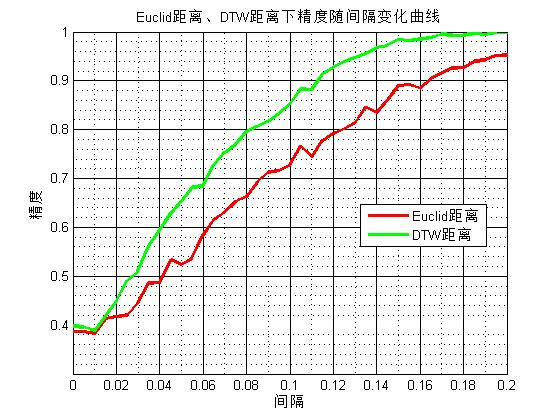
\includegraphics[width=\textwidth]{1.png}
      \caption{GP预测及谱密度示意图}\label{1}
    \end{figure}

\end{enumerate}

\section*{下周计划}
\begin{itemize}
  \item 继续看LDA相关知识,看MLAPP,处理课后习题,看看优化相关的论文。
\end{itemize}

\end{document} 